\chapter{Kapcsolódó megoldások}

\section{Technológiák bemutatása}
% bevezetes ilyen modszere altal transf

A modern szövegelemzési és nyelvfeldolgozási módszerek az elmúlt évtizedben jelentős fejlődésen mentek keresztül, ami elsősorban a transformer architektúrának és az előtanított nagy nyelvi modelleknek köszönhető \cite{transformer}. A szóvektorokra építő folyamatokat felváltotta az általános nagy nyelvi modellek feladatspecifikus finomhangolása.

\subsection{BERT}

2018-ban nagy áttörést jelentett a természetes nyelvű szövegelemzés területének a transformer architektúrát alkalmazó BERT modell megjelenése \cite{bert}. Ez encoder mechanizmust használ a szöveg reprezentálására, ami képes többek között klasszifikációs, névelem felismerés és kérdés-válaszolás feladatok megoldására is.

Nagy áttörést jelentett 2020-ban a magyar nyelvű szövegelemzés számára az első magyar nyelvű BERT modell, a huBERT \cite{Nemeskey:2021a} megjelenése. Ez egy BERT-Base típusú modell, ami 9 milliárd tokent tartalmazó magyar nyelvű szövegen lett tanítva. Számos magyar nyelvi benchmarkon jobban teljesít, mint a több-nyelvű BERT modellek.

\subsection{GPT}

A nagy nyelvi modellek következő generációját a szöveggenerálási feladatra tanított GPT modellek jelentették \cite{gpt1}. Ezek szintén a transformer architektúrát használják, viszont az encoder oldal mellett egy decoder-t is tartalmaznak. A BERT-el ellentétben ezt csak a következő token megtippelésre tanították, viszont szöveggeneráló képessége miatt képes sokféle feladatot elsajátítani finomhangoláson keresztül \cite{gpt2}.

A generatív nyelvi modellek közt nagy újításnak számított a GPT-3, melyről kiderült, hogy finomhangolás nélkül is képes feladatokat megoldani néhány példa (few-shot) alapján vagy akár példák nélkül (zero-shot) is \cite{gpt3}. Ennek a felfedezésnek a továbbviteleként született az InstructGPT, ami természetes nyelven megfogalmazott instrukciók/kérdések megválaszolására lett finomhangolva \cite{instructgpt}. A GPT-3 és az InstructGPT utódjaiként a GPT-4 és a ChatGPT sokat javítottak elődjeikhez képest, már szinte emberi szinteken teljesítve több feladatban is \cite{gpt4}.

\subsection{LoRA}

Ahogy nagy nyelvi modellek egyre elterjedtebbé váltak az utóbbi pár évben, megnőtt az igény ezeknek a finomhangolására, de egy klasszikus finomhangolás hosszú és erőforrásigényes procedúra. Ennek orvoslására találták ki a LoRA \cite{hu2022lora} finomhangolást, ami befagyasztja az előtanított nyelvi modell súlyait és annak kiválasztott részeit módosítja csak. A finomhangolás ezen kiválasztott súlyokat tartalmazó mátrixokat dekomponálja két kisebb mátrixszá, ezzel tovább csökkentve a hangolandó paramétereke számát. Ez a technika a hagyományos módszerhez képest akár harmadára is csökkentheti a szükséges memóriahasználatot és jóval kevesebb időt vesz igénybe.

\begin{figure}[H]
	\centering
	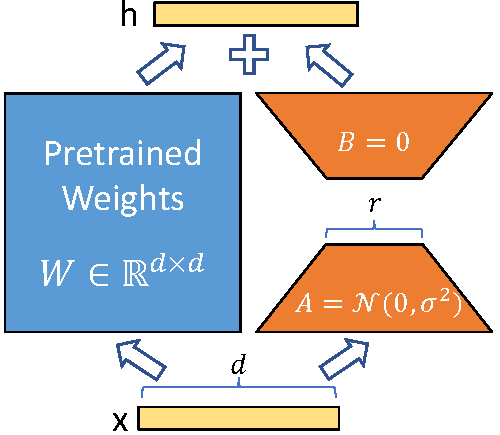
\includegraphics[width=0.49\textwidth]{figures/figure1.pdf}
	\caption{LoRA működése \cite{hu2022lora}}
\end{figure}

A LoRA használata a kisebb erőforrásigényen kívül azzal az előnnyel is jár, hogy a finomhangolás során keletkezett LoRA adapterek (súly módosítások) kevés helyet foglalnak a memóriában. Ha az alap modell már be van töltve a LoRA részek gyorsan cserélhetők futás közben, így megtehetjük, hogy feladatonként külön LoRA adaptert hangolunk és futás közben váltogatunk köztük.

Habár a technológia eredetileg nyelvi modellekhez lett kitalálva, képgeneráló modellekhez is adaptálták.

\subsection{QLoRA}

A LoRA módszerre épitve kutatók további fejlesztéseket dolgoztak ki LoRA adapterek hangolására alacsonyabb erőforrásigény elérése céljából a modell súlyainak kvantizálásával. A súlyok kvantizálása tömörítésként is felfogható és nagy (nyelvi) modelleknek arra a jól ismert tulajdonságára épít, hogy a súlyaik pazarló (nem optimális) módon tárolnak információt.

A QLoRA három fő innovatív módszer kombinációja:
\begin{enumerate}
	\item \textbf{4-bites NormalFloat}: kvantizációhoz használt adattípus, ami bizonyítottan optimális normál eloszlású súlyok esetén
	\item \textbf{Dupla Kvantizálás} (Double Quantization): egy módszer, ami a kvantizációs konstansokat kvantizálja, ezzel átlagosan 0.37 bitet spórol meg paraméterenként
	\item \textbf{Lapozott Optimalizálók} (Paged Optimizers): a neurális hálók optimalizáláshoz szükséges memória egy részét RAM-ban tárolja időlegesen, amivel a hosszabb szövegek miatti hirtelen memória-ingadozás esetén bekövetkező memória-túllépést ki lehet küszöbölni
\end{enumerate}

A QLoRA leglényegesebb újítása a LoRA-hoz képest tehát az, hogy az eredeti modell súlyait 4 bites számokkal tölti be 16 bit helyett, viszont közben az adaptert 16 biten hangolja.

\subsection{transformers (könyvtár)}

A transformers könyvtár \cite{transformers} egy egyszerű fejlesztői felületet ad, amin keresztül könnyen használhatók előtanított modellek háttérrendszertől (PyTorch, TensorFlow, JAX) függetlenül. A használat mellett a szoftvercsomag finomhangolást is támogat a legfrissebb fejlesztéseket (LoRA, QLoRA) beépítve. 

A könyvtár fejlesztői egy modellek és adathalmazok megosztását lehetővé tevő platformot is létrehoztak Hugging Face Hub néven. Ez a transformers-be integrálva egyszerűen hozzáférhetővé tett rengeteg különböző modellt fejlesztők számára.

\subsection{llama.cpp}

A transformer architektúra, amit a nagy nyelvi modellek többsége követ párhuzamosítható műveletek végzésére épül és emiatt leghatékonyabban videokártyákon (vagy speciális hardware-en) használható. Azonban GPU-k bérlése költséges és egyes alkalmazásoknál nem jelent problémát a késleltetés.

A llama.cpp egy generatív nyelvi modellek (elsősorban) processzoron való futtatására optimalizált szoftver. Alacsony szintű C/C++ nyleven lett fejlesztve és külön optimalizálták az egyes CPU architektúrákra, támogatva a SIMD operációkat.

\subsection{SpaCy}
Szövegek nyelvtani elemzésére számos módszert kidolgoztak, ezeknek egységesítésére jött létre a SpaCy \cite{spacy} Python könyvtár, ami fejlesztőknek nyújt egy kényelmes felületet. Az eszköztárában vannak minta alapú, konvolúciós neurális hálót alkalmazó és transzformer modelleket használó megoldások is.

A SpaCy bővíthető és magyar nyelvre is készült hozzá bővítmény, ez a HuSpaCy \cite{huspacy} . A HuSpaCy-nek több variációja is elérhető, az ezek közti különbség a háttérben használt modell architektúrájából fakad. A gyakorlatban ezek választásával a pontosság és hatékonyság között lehet egyensúlyozni.

A statisztikai alapú modellek valójában semmit nem érnek jó minőségű adat nélkül, ezen forrásokat is muszály megemlíteni:
\begin{itemize}
	\item UD Hungarian Szeged \cite{ud-hungarian-szeged} \cite{vincze-etal-2010-hungarian}
	\item NYTK-NerKor Corpus \cite{nerkor}
	\item Szeged NER Corpus \cite{szarvas-etal-2006-highly}
\end{itemize}

\section{Hasonló munkák}
% kepek ezekbol ertekeles miben jo adatok minoseg
\subsection{JaMIE: A Pipeline Japanese Medical Information Extraction System \cite{jamie}}

Információ kinyerő rendszerek egyik népszerű alkalmazása egészségügyi szövegek elemzése. A JaMIE rendszer egy három lépésből álló csővezeték architektúrát követ. Ez a rendszer entitásokra koncentrál, a felismerés után modalitás szerinti klasszifikációt futtat rajtuk, majd kinyeri a köztük fennálló kapcsolatokat. A feladaton két modellt hasonlítanak össze: BERT és LSTM + word2vec, minden benchmark esetében a BERT teljesít jobban.

\begin{figure}[H]
	\centering
	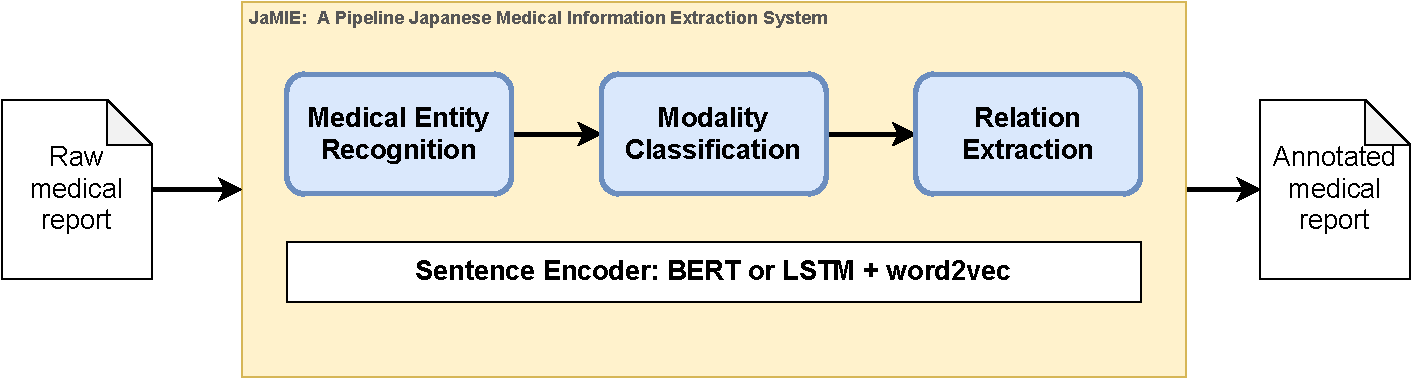
\includegraphics[width=1\textwidth]{figures/jamie.pdf}
	\caption{JaMIE működési folyamata \cite{jamie}}
\end{figure}

\subsection{Exploring the Potential of Twitter to Understand Traffic Events and Their Locations in Greater Mumbai, India \cite{twitter-traffic}}

Az információ kinyerés egy másik alkalmazása a Twitter platformon megosztott közúti balesetek valós idejű gyűjtése vagy ábrázolása. Ehhez a szerzőpáros első lépésként klasszifikálta a friss tweet-eket, majd kinyerték belőlük a névelemeket, kifejezetten a helyszínt. A klasszifikációhoz több klasszikus modellt is összehasonlítottak, melyek közül az SVM bizonyult leginkább ígéretesnek. A helyszínek kinyerésére egy kész megoldást - a StanfordNER-t - kombinálták egy saját adatukon tanított OpenNLP modellel és szabályalapú módszerekkel.

\subsection{RESIN \cite{resin}}

Egy másik terület, ahol hasonló információ kinyerő feladatról lehet beszélni: a hírek elemzése. A RESIN egy olyan rendszer, ami többféle nyelven írt szövegekből, de akár videós anyagokból képes entitásokat és történéseket kinyerni. Az entitások, valamint a köztük fennálló kapcsolatok kinyeréséhez BERT modellt használtak. Események kinyeréséhez dokumentum szinten alkalmazták a BART modellt. Az entitásokat és eseményeket a koreferencia feloldás mellett hozzákötötték a WikiData nevű tudásbázishoz. A megoldás érdekessége, hogy mindezt egy egyszerűen telepíthető Docker konténerként tették elérhetővé GitHub-on.

\begin{figure}[H]
	\centering
	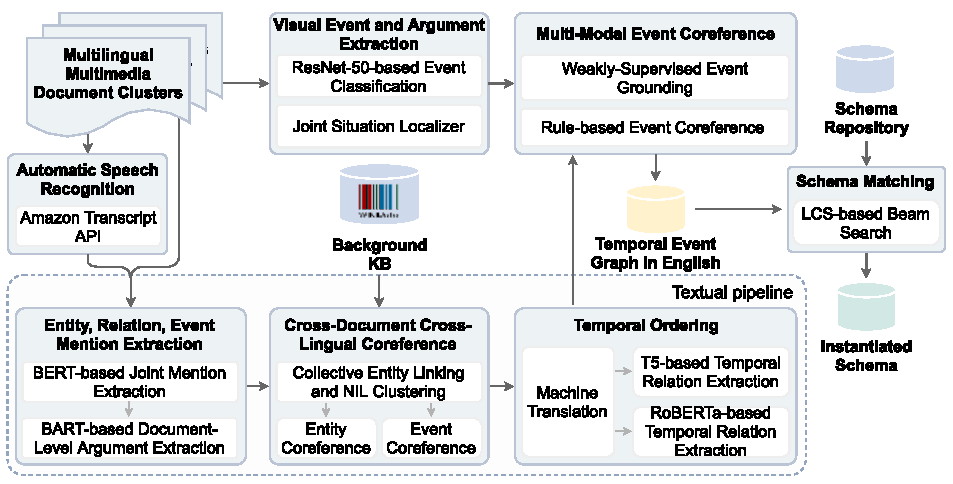
\includegraphics[width=1\textwidth]{figures/resin.pdf}
	\caption{RESIN működési folyamata \cite{resin}}
\end{figure}

% \subsection{Klasszikus módszerek}
% nem  kell
% Egyik első technika szöveg vektorrá alakítására a BoW (Bag of Words) tokenizáció volt, ami a szavak előfordulási gyakoriságát használja, viszont azok sorrendiségét teljesen figyelmen kívül hagyja. Ennek a továbbfejlesztése az N-gram modell, ami már szópárokban gondolkodik, így pontosabban képes szókapcsolatokat reprezentálni. Klasszifikációs feladatoknál még nagy javulást jelentett a TF-IDF módszer. Ez aszerint súlyozza az egyes kifejezéseket, hogy mekkora azok előfordulási aránya az aktuális dokumentumban és az összes dokumentum között.

% A neurális hálók elterjedése a szövegelemzés más területeihez hasonlóan itt is nagy áttörést jelentett. Már a konvolúciós hálók is képesek voltak jobb eredményt elérni a klasszikus módszereknél.